\chapter{Response Theory and Molecular Properties}\label{ch:molprop}

\begin{epigraphs}
\qitem{
White light goin' messin' up my brain

White light it's gonna drive me insane
}{
--- \textsc{The Velvet Underground}
}
\qitem{What's the frequency, Kenneth? [...]

          I never understood the frequency, uh-huh}{
          --- \textsc{R.E.M.}}
\end{epigraphs}

Response theory provides an \emph{ab initio} framework for the
formulation and computation of molecular properties and can be
considered the connection between quantum chemistry and experimental
chemistry.
The response treatment of molecular properties has its roots in
time-dependent perturbation theory\autocite{Konishi2009-zb} and has been
continually developed in quantum chemistry for the past 30
years.\autocite{Olsen1985-nr, Helgaker1992-ph, Olsen1995-pf,
Christiansen1998-pe, Norman2011-ad, Helgaker2012-cz, Pawlowski2015-sq}

Section \ref{sec:exact-response} will give a brief introduction to exact
state response theory for isolated molecules. The concepts of
quasienergy,\autocite{Christiansen1998-pe} variational perturbation
theory\autocite{Helgaker1992-ph} and pole-and-residue
analysis of response functions\autocite{Olsen1985-nr} will be introduced.
The exposition closely follows the one by \citeauthor{Saue2002-ns}
in \noparcite[ref.][]{Saue2002-ns}.
I will explicitly derive the \acrshort{SCF} response function for a
quantum/classical polarizable Hamiltonian in Section
\ref{sec:csm-response}. The derivation will employ the
density matrix-based, \acrshort{AO} formalism introduced by
\citeauthor{Thorvaldsen2008-sg} in \noparcite[ref.][]{Thorvaldsen2008-sg}.
This formalism is suitable for the derivation of arbitrary-order
response functions and their residues, also when perturbation-dependent
basis sets are considered.\autocite{Friese2015-kb, Friese2015-bu}
\paper{V} presents the arbitrary-order derivation of the \acrshort{PCM}.

\section{Exact State Response Theory}\label{sec:exact-response}

Let us consider the experimentally relevant situation where a molecular
system is subject to an external source of electromagnetic radiation.
Here and in the following, "external" will be used to mean an
electromagnetic field which is "weak" when compared to the
electron--electron and electron--nuclei interactions in the molecule.

\begin{figure}[tb]
  \centering
  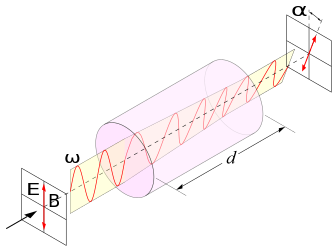
\includegraphics[width=.5\textwidth]{Optical-rotation.png}
  \caption{
  When a molecular system is subject to an external electromagnetic
  radiation of frequency $\omega$, a macroscopic, experimentally
  measurable response can be detected.
  Intensity and position of the signal can be related to the microscopic
  detail of the molecular system, as described by quantum mechanics.
  The picture depicts an optical rotation experiment where
  the linear polarization of the incident electromagnetic field
  is rotated by an angle $\alpha$ upon traversing a chiral material.
  Reproduced, with modifications, from \href{https://commons.wikimedia.org/wiki/File:Optical-rotation.svg}{Wikipedia}.
  }
  \label{fig:OR}
\end{figure}

The system can then be described by means of a combined matter--field
Hamiltonian:
\begin{equation}
  H = H_\mathrm{matter} + H_\mathrm{field} + H_\mathrm{int},
\end{equation}
where the three terms describe the molecular sample, the electromagnetic
field and their interaction, respectively.
Since our focus is on the molecular system, one can neglect the
quantized description of the field and treat the interaction term in a
semiclassical fashion.\autocite{Craig2012-zp}
The time-dependent Schr\"{o}dinger equation is now the appropriate
equation of motion:
\begin{equation}\label{eq:td-schrodinger}
  H\psi(t) = \mathrm{i}\pderiv{\psi(t)}{t},
\end{equation}
where the time-dependent, semiclassical matter--field Hamiltonian is
used:
\begin{equation}
  H = H_0 + V(t).
\end{equation}
The perturbation is a one-electron operator. We will further assume that
it is periodic in time $V(t) = V(t+T)$ and admits a discrete Fourier
decomposition:
\begin{equation}\label{eq:fourier}
  \begin{aligned}
 V(t) &=
 \sum_{k=-N}^N \expo{-\mathrm{i}\omega_k t}V(\omega_k)
 =
 \sum_{k=-N}^N\expo{-\mathrm{i}\omega_k t} \sum_X \epsilon_X(\omega_k)V_X \\
 &=
 \sum_{x}\expo{-\mathrm{i}\omega_x t}\epsilon_x V_X
  \end{aligned}
\end{equation}
where all the frequencies are integer multiples, $\omega_k=n_k \omega$
of the fundamental frequency $\omega = \frac{2\pi}{T}$.\autocite{Olsen1985-nr}
Frequencies and amplitudes in the Fourier decomposition obey the
following relations:
\begin{alignat}{2}
 \omega_{-k} = \omega_{k},
 \quad&
 \epsilon_x = \epsilon_X^*(\omega_k)
 =
 \epsilon_X(\omega_{-k}) = \epsilon^*_{-x},
\end{alignat}
since the $V(t)$ is required to be Hermitian.
For notational convenience, the perturbation operator ($X$) and
frequency ($k$) indices have been collapsed into the common index $x$.

Under the assumption that the external field is weak with respect to the
molecular field, time-dependent perturbation theory is an appropriate
tool to approximately solve Eq. \eqref{eq:td-schrodinger}.
The response theory route to molecular properties introduces a
phase-separated ansatz for the time-dependent wave function:
\begin{equation}\label{eq:phase-separated}
  \psi(t) = \expo{-\mathrm{i}F(t)}\bar{\psi}(t),
\end{equation}
where the time-derivative of the phase factor defines the time-dependent
\emph{quasienergy}:\autocite{Christiansen1998-pe, Pawlowski2015-sq}
\begin{equation}
  Q(t) = \dot{F}(t) = \Braket{\bar{\psi}(t) |
  H_0 + V(t) - \mathrm{i}\pderiv{}{t}
  | \bar{\psi}(t)}.
\end{equation}
The time-dependent quasienergy is variational, but the corresponding
time-dependent Hellmann--Feynman theorem cannot straightforwardly be
applied to the calculation of molecular properties. Fortunately, we can exploit the
periodicity of the perturbation operator to introduce the time-averaged
quasienergy:
\begin{equation}
  \aveQ =
 \frac{1}{T} \int_{-\frac{T}{2}}^{\frac{T}{2}} \diff t Q(t) =
 Q_0 + \sum_{x}\epsilon_x E_x
\end{equation}
where:
\begin{subequations}
 \begin{align}
  Q_0 &= \left\lbrace \Braket{\bar{\psi}(t) | H_0 | \bar{\psi}(t)} \right\rbrace_T
- \left\lbrace \Braket{\bar{\psi}(t) | \mathrm{i} \pderiv{}{t} | \bar{\psi}(t)}\right\rbrace_T = E_0(0) - S \\
  E_x &= \left\lbrace \Braket{\bar{\psi}(t) | V_X | \bar{\psi}(t)}\exp(-\mathrm{i}\omega_k t) \right\rbrace_T
 \end{align}
\end{subequations}
Differentiating the time-averaged quasienergy yields the time-averaged
Hellmann--Feynman theorem:
\begin{equation}\label{eq:tave-hellfeyn}
  \deriv{\aveQ}{\epsilon_X(\omega_k)}
  =
  \left\lbrace\Braket{\bar{\psi}(t) | \pderiv{H}{\epsilon_x} | \bar{\psi}(t)}\right\rbrace_T
  = E_x,
\end{equation}
which can be used to connect response functions to molecular properties.
Letting $\ket{0}$ represent the unperturbed reference state, we can
develop the Kubo expansion at zero perturbation strength of the
expectation value of the observable $H_X$:\autocite{Kubo1957-ay}
\begin{equation}
\begin{aligned}
 \Braket{\bar{\psi}(t) | V_X | \bar{\psi}(t)} &\simeq
 \Braket{0|V_X|0} +\sum_{k=-N}^N
 \response{V_X}{V(\omega_k)}{\omega_k}\expo{-\mathrm{i}\omega_k t} \\
 &+\frac{1}{2}\sum_{k,l=-N}^N
 \response{V_X}{V(\omega_k),V(\omega_l)}{\omega_k,\omega_l}\expo{-\mathrm{i}(\omega_k+\omega_l)t}
\end{aligned}
\end{equation}
response functions may be identified as the Fourier coefficients in the
expansion. These are none other but higher order derivatives of the
time-averaged quasienergy, as a comparison with the same expansion for
the right-hand side of Eq. \eqref{eq:tave-hellfeyn} will confirm:
\begin{equation}\label{eq:kubo}
\begin{aligned}
  \deriv{\aveQ}{\epsilon_x}
  &\simeq \Braket{0|V_X|0}\delta_{\omega_x} \\
  &+\sum_{y}\response{V_X}{V_Y}{\omega_y}\epsilon_y\delta_{\omega_x+\omega_y} \\
  &+\frac{1}{2}\sum_{y,z}\response{V_X}{V_Y,V_Z}{\omega_y,\omega_z}\epsilon_y\epsilon_z\delta_{\omega_x+\omega_y+\omega_z}
\end{aligned}
\end{equation}
First and higher order molecular properties can now be identified from
the response functions appearing as Fourier coefficients in the Kubo
expansion by taking the appropriate perturbation-strength derivatives at
zero field strength:
\begin{equation}\label{eq:nth-order-derivative}
  \left.\frac{\diff^n \aveQ}{\diff\epsilon_{x_1}\diff\epsilon_{x_2}\cdots\diff\epsilon_{x_n}} \right|_{\vect{\epsilon}=0}
  =
  \response{V_{X_1}}{V_{X_2}, \ldots, V_{X_n}}{\omega_{x_2},\ldots,\omega_{x_n}}\delta_{\omega_{x_1}+\cdots+\omega_{x_n}},
\end{equation}
the $\delta_{\omega_{x_1}+\cdots+\omega_{x_n}}$ notation is used to
enforce the sum rule on the probing and response frequencies involved in
the expansion:
\begin{equation}\label{eq:sum-rule}
 \sum_{i=1}^{n} \omega_{k_i} = 0
\end{equation}
%\begin{subequations}
%  \begin{align}
%  \left.\deriv{\aveQ}{\epsilon_a}\right|_{\vect{\epsilon}=0} &= \Braket{0|V_A|0}\delta_{\omega_a} \\
%  \left.\frac{\diff^2 \aveQ}{\diff\epsilon_a\diff\epsilon_b}\right|_{\vect{\epsilon}=0}
%         &=
%         \response{V_A}{V_B}{\omega_b}\delta_{\omega_a+\omega_b} \\
%  \left.\frac{\diff^3\aveQ}{\diff\epsilon_a\diff\epsilon_b\diff\epsilon_c}\right|_{\vect{\epsilon}=0}
%  &=
%  \response{V_A}{V_B, V_C}{\omega_b,
%  \omega_c}\delta_{\omega_a+\omega_b+\omega_c}.
%  \end{align}
%\end{subequations}
Response functions quantify how, to a certain order in the perturbing
field tuples, the expectation value of a given observable is modified.
The semicolon appearing in the response functions separates the operator
$V_X$, whose response is measured, from the external perturbations
$V_Y$, $V_Z$\dots{} causing it.
From the perturbation expansion Eq. \eqref{eq:kubo}, it is clear that
permutation symmetry exists between the external perturbations provided
that the corresponding frequencies are permuted concomitantly.

Having introduced response functions as a useful tool to quantify the
effect of external perturbations on molecular properties, it is now time
to consider how to actually compute them.
In this Section, we are concerned with exact wave functions that can
thus be parametrized in a variational fashion by a set of parameters
$\vect{\lambda}$: $\ket{0}=\ket{0(\vect{\lambda})}$.
We recall that the Lagrangian method outlines in Section
\ref{sec:coupled-cluster} can be employed also in this
case.\autocite{Christiansen1998-pe, Helgaker2012-cz, Pawlowski2015-sq}
The optimal parameter set is determined upon minimization of the
time-averaged quasienergy:
\begin{equation}\label{eq:var-cond}
 \deriv{\aveQ}{\vect{\lambda}} = 0.
\end{equation}
In variational perturbation theory,\autocite{Helgaker1992-ph,
Saue2002-ns} we assume the variational parameters to be functions of the
perturbation strength parameters: $\vect{\lambda} =
\vect{\lambda}(\vect{\epsilon})$.
Furthermore, we require the stationarity condition to hold at \emph{all}
perturbation strengths, with $\lambda(0) = 0$, for convenience.

The perturbation-strength total derivative at zero perturbation strength
of the time-averaged quasi energy is:
\begin{equation}
\begin{aligned}
 \left[\prod_{i=1}^n \deriv{}{\epsilon_{x_i}}\right]\aveQ
 &= Q^{[n]}_{x_1 \ldots x_n}
 =
 Q^{[n]}_{0; x_1 \ldots x_n}
 + \sum_{j=1}^{n}E^{[n-1]}_{x_j;x_1\ldots x_{j-1}x_{j+1}\ldots x_n} \\
 &=
 \left[\prod_{i=1}^n \deriv{}{\epsilon_{x_i}}\right]Q_0
 + \sum_{j=1}^n
 \left[\prod_{i\neq j}^{n-1} \deriv{}{\epsilon_{x_i}}\right]E_{x_j}
\end{aligned}
\end{equation}
Notice that this is just an alternative and more verbose notation for
Eq. \eqref{eq:nth-order-derivative}, which allows to express response
functions in terms of wave function perturbed parameters.
%for first and second-order properties one has:
%\begin{subequations}
% \begin{align}
%   Q^{[1]}_{a} &= \left[Q^{[1]}_{0; a} + E_{a}\right]\delta_{\omega_a} =
%   \braket{0| V_A | 0}\delta_{\omega_a} \\
%  Q^{[2]}_{ab} &= \left[Q^{[2]}_{0; ab} + E^{[1]}_{a;b} + E^{[1]}_{b;a}\right]\delta_{\omega_a+\omega_b}
%  = \response{V_A}{V_B}{\omega_b}\delta_{\omega_a+\omega_b}
% \end{align}
%\end{subequations}
Application of the chain rule to the total derivatives in fact yields:
\begin{subequations}
 \begin{align}
   Q^{[1]}_{a} &=
   \sum_{\sigma}\left[
   Q^{[1]}_{0; \sigma}\lambda^{[1]}_{\sigma;a} + E_{a}
   \right]\delta_{\omega_a} \\
   Q^{[2]}_{ab} &=
   \sum_{\sigma\tau}\left[
   \lambda^{[1]}_{\sigma;a}Q^{[2]}_{0;\sigma\tau}\lambda^{[1]}_{\tau;b}
   + Q^{[1]}_{0; \sigma}\lambda^{[2]}_{\sigma;a}
   + E^{[1]}_{a;\sigma}\lambda^{[1]}_{\sigma;b}
   + E^{[1]}_{b;\sigma}\lambda^{[1]}_{\sigma;a}
   \right]\delta_{\omega_a+\omega_b} \label{eq:linres}
 \end{align}
\end{subequations}
where the following tensors were introduced:
\begin{subequations}
 \begin{align}
 Q^{[n]}_{0; \sigma_1\cdots \sigma_n} &=
 \frac{\partial^n Q_0}{\partial\lambda_{\sigma_1}\cdots\partial\lambda_{\sigma_n}} \\
 E^{[n]}_{x;\sigma_1\cdots \sigma_n} &=
 \frac{\partial^n E_x}{\partial\lambda_{\sigma_1}\cdots\partial\lambda_{\sigma_n}} \\
\lambda^{[n]}_{\sigma;x_1\dots x_n} &=
\frac{\partial^n \lambda_\sigma}{\partial \epsilon_{x_1}\cdots\partial \epsilon_{x_n}}
 \end{align}
\end{subequations}

The response equations, determining the $\vect{\lambda}^{[n]}$ tensor of
perturbed wave function parameters, are obtained by differentiating the
variational condition on the time-averaged quasienergy Eq.
\eqref{eq:var-cond}:\autocite{Olsen1985-nr, Helgaker1992-ph, Christiansen1998-pe}
\begin{equation}
 R_{\sigma;x_1\cdots x_n}^{[n]} = \left[\prod_{i=1}^n \deriv{}{\epsilon_{x_i}}\right]
\left. \deriv{\aveQ}{\lambda_\sigma}\right|_{\vect{\epsilon}=0} = 0.
\end{equation}
The determination of second-order properties requires the knowledge of
the first-order response of the wave function:
\begin{subequations}
 \begin{align}
 R_{\sigma}^{[0]} &= Q_{0;\sigma}^{[1]} = 0 \\
 R_{\sigma;a}^{[1]} &= \sum_{\tau}Q_{0;\sigma\tau}^{[2]}\lambda_{\tau;a}^{[1]} + E_{a;\sigma}^{[1]} = 0.
 \label{eq:1st-order-response}
 \end{align}
\end{subequations}
The time-averaged quasienergy formalism allows to formulate response
properties to static and dynamic fields on an equal footing as
perturbation-strength derivatives.
Moreover, variational perturbation theory achieves a transparent
derivation of the necessary response equations.\autocite{Helgaker1992-ph}

Let us consider in more detail the form of the linear response function
Eq. \eqref{eq:linres}. The formal solution to the response equation Eq.
\eqref{eq:1st-order-response} can be obtained by inverting the
\emph{Hessian}. Eq. \eqref{eq:linres} can then be rewritten as:
\begin{equation}
  \response{V_A}{V_B}{\omega_b}
  =
   -\sum_{\sigma\tau}
   E^{[1]}_{a;\sigma}
   \left[\mat{Q}^{[2]}_{0}\right]^{-1}_{\sigma\tau}
   E^{[1]}_{b;\tau}.
\end{equation}
Expansion into the exact eigenbasis of $H_0$ yields the
\gls{SOS} expression for the linear response function:
\begin{equation}
  \response{V_A}{V_B}{\omega_b}
  =
  -\sum_{n>0}\left[
  \frac{\braket{0|V_A|n}\braket{n|V_B|0}}{\omega_{n0}-\omega_b}
  +
  \frac{\braket{0|V_B|n}\braket{n|V_A|0}}{\omega_{n0}-\omega_a}
  \right]\delta_{\omega_a+\omega_b}.
\end{equation}
The excitation energies of the system appear in the denominators
$\omega_{n0} = E_n - E_0$ and can thus be identified as the \emph{poles}
of the response function. Moreover, the \emph{residues} at
the poles are the transition moments determining the intensity of
spectroscopic transitions:
\begin{equation}
  \lim_{\omega_b\rightarrow\omega_{n0}}
  \response{V_A}{V_B}{\omega_b}
  = \braket{0|V_A|n}\braket{n|V_B|0}.
\end{equation}
A similar analysis holds also for higher order response functions. The
pole structure of the higher order quantities also conveys information
about the excited states \emph{via} single and double
residues.\autocite{Olsen1985-nr, Christiansen1998-pe, Helgaker2012-cz}

\section{SCF Response Theory for Quantum/Classical Polarizable Hamiltonians}\label{sec:csm-response}

\acrshort{PCM}~\autocite{Cammi1994-qj, Cammi1996-wf, Cammi1996-vx,
Cammi1999-rb, Cammi2003-qy, Frediani2005-nc, Ferrighi2010-pm}
\acrshort{FQ} and \acrshort{FQ}/\acrshort{PCM}~\autocite{Lipparini2012-hx, Lipparini2012-tl, Lipparini2013-ud}
\acrshort{PE}~\autocite{Olsen2010-wa}
\acrshort{QM}/\acrshort{MM}/Continuum~\autocite{Steindal2011-ki, Caprasecca2012-ir}
Open-ended \acrshort{AO}-based \acrshort{SCF} response~\autocite{
Larsen2000-hj, Kjaergaard2008-hy, Thorvaldsen2008-sg,
Kristensen2008-hv, Ringholm2014-gx}
Open-ended \acrshort{SCF} residues~\autocite{Friese2015-kb}
\paper{V}\autocite{pcm-openrsp}
Solution strategy for response equations~\autocite{Saad2003-oa,
Saad2011-gm, Kauczor2011-rd, Malmqvist2013-vw}

